%\documentclass[10pt,a4paper]{article}

\documentclass[24pt]{article}

\usepackage{arxiv}
\usepackage[utf8]{inputenc} % allow utf-8 input
\usepackage[T1]{fontenc}    % use 8-bit T1 fonts
\usepackage{hyperref}       % hyperlinks
\usepackage{url}            % simple URL typesetting
%\usepackage{booktabs}       % professional-quality tables
\usepackage{amsfonts}       % blackboard math symbols
\usepackage{nicefrac}       % compact symbols for 1/2, etc.
\usepackage{microtype}      % microtypography
\usepackage{lipsum}         % Can be removed after putting your text content
\usepackage{graphicx}
\usepackage{natbib}
\usepackage{doi}
\usepackage{amssymb}
\usepackage{amsthm}
\usepackage{forest}


\usepackage{tikz} 
\usepackage{caption}
\usepackage{amsmath}
\usepackage{cleveref}       % smart cross-referencing
\usepackage{colortbl}
\usepackage{color}
\usepackage{listings}
\usepackage{multicol}
\usepackage{array}

\definecolor{orange151}{rgb}{0.9,0.647,0}
\definecolor{lgreen}{rgb}{0.564,0.93,0.564}


\usepackage{color}

\definecolor{dkgreen}{rgb}{0,0.6,0}
\definecolor{gray}{rgb}{0.5,0.5,0.5}
\definecolor{mauve}{rgb}{0.58,0,0.82}

\lstset{frame=none,
  language=Python,
  aboveskip=3mm,
  belowskip=3mm,
  showstringspaces=false,
  columns=flexible,
  basicstyle={\small\ttfamily},
  numbers=none,
  numberstyle=\tiny\color{gray},
  keywordstyle=\color{blue},
  commentstyle=\color{dkgreen},
  stringstyle=\color{mauve},
  breaklines=true,
  breakatwhitespace=true,
  tabsize=3
}
\definecolor{dgreen}{rgb}{0,0.5,0}
\definecolor{bg}{rgb}{0.125,0.51,0.49}
\definecolor{mag}{rgb}{0.866,0.627,0.866}
\definecolor{lgray}{rgb}{0.49,0.49,0.49}
\definecolor{dgray}{rgb}{0.82,0.788,0.827}
\definecolor{pink}{rgb}{1, 0.568, 0.686}
\definecolor{lblue}{rgb}{0.078, 0.741, 0.931}
\definecolor{orag2}{rgb}{0.87, 0.478, 0.12}

\newcommand*{\addheight}[2][.5ex]{%
  \raisebox{0pt}[\dimexpr\height+(#1)\relax]{#2}%
}

%\newcommand{\subf}[2]{%
%  {\small\begin{tabular}[t]{@{}c@{}}
%  #1\\#2
%  \end{tabular}}%
%}

\newtheorem{theorem}{Theorem}[section]
\newtheorem{lemma}[theorem]{Lemma}
\newtheorem{proposition}[theorem]{Proposition}
\newtheorem{corollary}[theorem]{Corollary}
\newtheorem{example}[theorem]{Example}
\newtheorem{definition}[theorem]{Definition}


\title{Research methodology}

%\author{ \href{https://orcid.org/0000-0002-8749-3324}{
\includegraphics[scale=0.08]{orcid.pdf} \href{mailto: jacques.bourg739@gmail.com}{@}\hspace{1mm} Jacques Bourg    }}
\author{Jacques Bourg}


% Uncomment to override  the `A preprint' in the header
\renewcommand{\headeright}{}
\renewcommand{\undertitle}{}
\renewcommand{\shorttitle}{Snakes}


\hypersetup{
pdftitle={Research methodology}, 
pdfsubject={math.NT},
pdfauthor={Jacques Bourg},
pdfkeywords={Research methodology },
}
 

\begin{document}

\maketitle

\begin{abstract}

 
\end{abstract}

\keywords{ .}



\section{ d}
 
        ouiller les données.


        Processus 

        Fièvre

        La première chose est d'ordonner. Ordonner veut littéralement dire mettre dans le bon ordre. On peut par exemple partir de données et essayer de les visualiser de façons différentes. Je donne un exemple : l'orque l'on enregistre des neurones avec des électrodes ou avec des microscopes on arrive à isoler l'activité de neurones indépendants. L'activité de Chaque neurone correspond à une variable et on observe lors d'un enregistrementune centaine de variables simultanément.  Une façon de voir les données est donc d'ordonner les neurones selon un scalaire. Ce scalaire peut être l'activité moyenne, ou le rang du vecteur de la première composante principale, ou le rang de la corrélation entre deux neurones. Une fois les données triées, il est question de voir si cet ordre met en lumière une dynamique particulière des données. On pourra donc voir l'activité des neurones (dans le bon ordre) au cours du temps et voir si on trouve quelque dynamique particulière qui ne s'explique pas seulement par l'ordre que l'on a imposé: des oscillations au niveau de la population par exemple. 

        Sans ordre, sans une façon un peu particulière d'attaquer ou de voire un problème, je pense que c'est difficile de faire des progrès dans la compréhension que l'on en a, ou en tout cas de trouver quelque chose de nouveau.    Produire de la connaissance revient souvent à expliquer comment des choses connues s'imbriquent logiquement et sont intermelées. L'on invoque souvent d'ailleurs le rasoir d'occam comme un principe épistémologique qui va privilégier les hypothèses les plus simples. Celles CIS ne sont pas forcément vraies, mais ce sont celles que l'on doit examiner en premier.


        Rôle de la bibliographie: souvent lorsque l'on rentré dans un problème l'on peut être dépassé par toute la connaissance qui a été produite autour d'un problème. Les articles scientifiques sont parfois très difficiles à digérer, car ils condensent des années de travail.   Il convient donc de lire avec attention des articles qui soit donnent un aperçu général du domaine dans lequel on travaille, soit des articles qui sont proches de la problématique que l'on veut traiter. Ceux CIS donnent du vocabulaire,  les notions fondamentales à maîtriser et aussi une idée de l'extextension et la qualité que doit avoir un article scientifique.   Cependant, les questions spécifiques que l'on se pose, sont presque tout le temps, des problèmes auxquels personne n'a encore pensé ou des problèmes que l'on ne peut poser qu'au vu des dernières découvertes ( et donc des gens se les posent en même temps). 
        Lire des articles scientifiques est un exercice difficile  car il implique de comprendre les raisonnements de quelqu'un d'autre.    On peut, pour produire de la connaissance, ou du moins pour identifier une question de recherche, d'essayer de mettre à plat touts les briques de connaissance autour d'un sujet précis, et d'essayer d'y trouver des trous ou bien un cadre explicatif commun.

        Ce qu'il faut savoir, c'est que la disposition, l'état d'esprit qu'il faut pour faire de la bibliographie n'est pas du tout le même que celui qu'il faut pour écrire un code informatique ou celui de la réflexion pure. Par ceci je veux dire que ce ne sont pas les mêmes opérations mentales que l'on exécute. De la même façon que les sportifs font des échauffements, des exercices de précision et des sessions de tactique, le travail du chercheur est rythmé par des temps différents. Pour le chercheur débutant, en particulier, qui débute une thèse et qui n'a encore rien "trouvé", c'est à dire qui n'a pas de résultats à présenter, l'attente de l'eureka peut être fortement anxiogène, car il sait que trouver une question pertinente et/ ou un résultat initial encourageant ne constitue que la phase initiale de la recherche, qui doit aboutir à l'écriture d'un article de recherche.
        Il est primordial de garder la tête froide et d'aborder chaque phase avec un mélange de concentration et de relâchement.  


        Quand on assiste à un séminaire, ou que l'on lit un article, il faut oublier son sujet de recherche et essayer d'assimiler un contenu. Ces séminaires de recherche peuvent être très profitables si on s'y prend correctement, car ils permettent de se familiariser avec un domaine: quelles sont les tendances, comment se déroulent les expériences, comment critique t'on un protocole ? Quels sont les biais expérimentaux?


    Ne pas mélanger: pendant un séminaire de recherche il s'agit de comprendre certaines choses ( pas forcément tout). 
     



     



        et essayer d'assimiler ce que les autres chercheurs ont fait avec bienveillance et circonspection. On n'est pas obligés de croire
        aux résultats que l'on nous présente, mais l'attitude si souvent vue de dénigrer le travail des autres souvent pour se mettre en valeur alimente une.sorte de ressentiment et d'amertume que le chercheur développe et qui lui nuit profondément.




    La réfection. Comment faire advenir les idées ?





\section{Types de recherche}
 

Exploratoire


Descriptive




\section{Generer de nouvelles idées}



 

\subsection{Penser}
Penser vient du latin pensare qui litéralement veut dire peser ou apprécier. La pensée, comme la balance d'un maraîcher, est capable de produire des idées et de les soupeser afin de comparer leurs vertus et leurs défauts.  

Savoir écarter des idées est aussi important que de savoir identifier de bonnes idées. D'ailleurs, la penser quelque chose, c'est essayer de le voir sous un jour nouveau, et donc de tout mettre à plat et  de recommencer à assembler logiquement les pièces. Après avoir eu un ou deux eurekas, on sait ce que ça veut dire que de trouver quelque chose, on sait la simplicité et la beauté qui viennent avec une belle idée. On est donc en capable de tout remettre à plat et de reprendre à zéro un raisonement ou même un travail si on sent que la ligne directrice est trop compliquée.


Un fait absolument magique mais vrai est que la pensée arrive en pensant.  Si on est dans de bonnes dispositions mentales et physiques, les idées arrivent en travaillant et en prenant le temps, c'est aussi simple que ça.

Réfléchir, c'est travailler dans sa tête. 
Comme un rayon lumineux qui se réfléchirait sur des mirroirs, les idées se réfléchissent et tournent dans la tête, comme dans une réverbération. Cette réverbération s'obtient de diverses façons, que nous déveloperons successivement. 

\subsubsection{Ecrire}

    Un exercice qui peut être extrêmement profitable l'orque l'on réfléchit, c'est d'écrire. L'écriture doit d'être aussi  structurée que possible, comme s'il s'agissait d'écrire un chapitre de thèse, qui sera relu par quelques personnes. 
    Écrire de cette façon nous oblige à présenter avec précision des définitions et les questions de recherche auxquels on s'intéresse. Le temps de l'écriture étant beaucoup plus lent que celui de la pensée, écrire oblige la pensée à passer et repasser par les objets que l'on examine et à produire des énoncés précis.  Aussi, écrire est une très bonne façon de charger différents concepts dans sa mémoire de travail, et de commencer  à les faire jouer ensemble.

   
\subsubsection{Reproduire un résultat existant}









\subsection{Recherche à deux}:
Lors des revues hebdomadaires  avec le directeur de recherche ou l'encadrant, on a la possibilité d'exposer les avancées et les ecueils qu'on a rencontrées. 

La meilleure manière de le faire, même si ça à l'air un peu étrange, c'est de commencer ces entretiens par prendre du recul. Rappeller le contexte du problème que l'on est en train de résoudre, poser les hypothèses de recherche, les voies que l'on a explorées, ce qui n'a pas marché et ce qui a marché. Et ensuite sauter sur ce que l'on vient de faire depuis quelques semaines. 


Cette mise à distance, est en fait très difficile à faire, et parait un peu pesante car en tout cas pour le doctorant, il a le nez sur le sujet toute la journée. 
Par contre, ce n'est pas le cas pour l'encadrant, qui traite aussi d'autres sujets en parallèle. 
La difficulté de cette mise à distance réside dans la temporalité de la recherche: la recherche est relativement lente, et la quantité de travail produit d'une semaine à l'autre peut être relativement petite. 
Cette mise à distance peut bien sur être faite à des fréquences moindres, mais elle doit absolument être faite, car à force d'avoir le nez dans le guidon, on oublie les décisions qui ont été prises et on va manquer de hauteur. 

Suite au point sur le contexte de la recherche, l'on peut alors aller dans les détails. Parfois le fait de faire un calcul ensemble ou de montrer à l'étudiant comment procéder pour essayer des choses peut être très bénéfique: montrer que l'on procède à tatons et que l'important ce n'est pas d'arriver à trouver quelque chose de parfait, mais seulement quelque chose avec quoi travailler.


Pour un encadrant et un étudiant le fait d'avoir une intéraction périodique à un intêret pédagogique évident. Cependant, même dans le cas ou les chercheurs sont déjà formés et autonomes, faire de la recherche à deux peut être très bénéfique, car le processus de recherche est une sorte de va et vient entre produire des idées et les mettre à distance pour les évaluer. 

En résultat de ces entrevues, il convient toujours, comme lors de toute réunion de faire un plan d'actions: 
qu'est ce qui doit être fait, et la liste ne doit être ni trop longue, ni trop courte. 


\subsection{Tirer sur un fil}

Avant d'avoir une grande idée il est quand même très important de commencer quelque part. Après avoir identifié une idée comme étant raisonablement bonne, il faut essayer de l'exploiter et d'en tirer toutes ses conséquences. 





\subsection{Eureka}
Le processus long et douloureux qui précède une découverte consiste justement à faire jouer ensemble des concepts dans sa tête et d'essayer de les marier ensemble.  Ceci arrive de façon consciente, on écrit des textes, des équations, l'on explore différentes hypothèses pour voir ce qui marche et ce qui ne marche pas. C'est un processus douloureux justement parce que souvent rien ne marche, pendant très longtemps. On a l'impression de taper sa tête sur un mur.EtEnsuite, une fois que l'on a fini de travailler, le cerveau continue de travailler tout seul de façon inconsciente. C'est souvent d'ailleurs pendant 
    Les phases de relâchement que l'on voit les solutions et que le.moment eureka se produit, dans une explosion de joie ou d'excitation, ou peut être de soulagement. 







\subsection{La naiveté est un atout considérable}




\section{Avoir tout en tête}
Toutes les données du problème. 


\section{Entousiasme concentration en bien être}

Une très bonne recherche ne peut se faire que sans une très grosse dose d'entousiasme. Parfois cet enthousiasme relève du volontarisme, et c'est normal puisque parfois l'on doit passer par de longues phases assez éprouvantes voire fastidieuses de travail expérimental, par exemple. Il reste vrai que si l'on veut réussir, et le plus important, se sentir bien pendant les longues années de thèse, l'on doit trouver du plaisir dans ce que l'on fait. Si l'on arrive à tirer assez de plaisir et d'interêt pour ce que l'on fait on réussira à rester concentré pendant de longues heures, et le temps passera beaucoup plus vite que si vous vous déconcentrez en changeant souvent d'activité ou en allant sur internet pour vous changer les idées.

Sentir son cerveau réfléchir est extrêment plaisant. Déjà être capable de proposer des hypothèses, de les étudier et de faire des raisonnements cohérents est une source de stimulation. Mais, dès que vous aurez mis la main sur une idée un peu intérréssante et que vous tirerez sur le fil, alors votre cerveau se réveillera et vous sentirez vraiment le vertige et l'entousiasme monter et c'est là que vous devez y mettre toute votre energie  sans hésitation. 


\section{Questions expérimentales}

Poser une question. 

Est ce qu'on l'a bien posé ? 
Facteurs explicatifs.

Si je veux tester un papier, je 





\section{Questions théoriques}



\section{La bibliographie}
  
Role limitant ou stimulant. 


wittgensteinienne  "qui se serait vanté d’être le seul philosophe à Cambridge à n’avoir jamais lu une seule ligne d’Aristote"


La bibbli remplit des objectifs différents: 

-acquérir une culture du domaine. 

-apprendre à être critique avec les résultats (ceci s'apprend plutôt lors des séminaires). 

-voir comment sont structurées les études.


Enfin et seulement enfin. Dans la biblio, il y a cinq ou six papiers qui vont être intéressants pour le problème qu'on veut traiter, et qui contiennent des données de départ A, B, C, D, E qui vont nous permettre de produire le bout de connaissance F. Il faut voir A... comme des légos. De toutes petites pièces d'information. 


- Lire des papiers éternellement sans avoir défini une question relativement précise peut s'avérer être une perte de temps et d'energie considérables. Il convient donc de lire, mais avec des objectifs clairs en tête. Par exemple, au début de la thèse, on peut se donner le temps de lire des papiers juste pour comprendre la problématique et le domaine d'études. Une fois qu'on aura une problématique bien précise, on identifiera quelques papiers cléfs, et on distillera les connaissances essentielles qu'on a besoin pour essayer de résoudre un problème. 


Enfin, lors de l'écriture d'un article scientifique ou de la thèse, on lit des papiers pour faire une bonne introduction, c'est à dire établir le contexte scientifique dans lequel notre étude vient s'inscrire. Par exemple, c'est très utile de pouvoir grouper des études par thématique, méthodologie ou façon d'aborder le problème. Si possible c'est très utile de pouvoir cartographier ce qui à été fait dans un domaine, et de pouvoir identifier les régions inexplorées: c'est néanmoins assez difficile et c'est plutôt à l'encadrant ou au directeur de thèse qui souvent ont proposé le sujet  , d'avoir ce recul.


- 

\section{Système de récompense}

Il est parfois difficile de garder sa motivation lorsque les buts à atteindre sont assez éloignés dans le temps et comportent une part d'aléatoire. Le fait d'obtenir des bons résultats, d'écrire un papier de recherche, de publier dans de bonnes revues ou même d'envisager une carrière académique, sont des objectifs qui ne peuvent pas s'obtenir sur le court terme. Il convient donc de baser son effort, sa concentration et son ressenti  sur le travail que l'on fournit quotidiennement. L'on doit se fixer des objectifs assez limités dans le temps: réussir d'abord à faire les choses les plus élémentaires, comme des expériences, des calculs ou des présentations, et essayer de mesurer ses performances seulement sur ces critères, afin de baser son système de récompense sur sa  progression et non sur des événements qui ne sont pas encore arrivés.  
Un autre facteur de plaisir consiste à redoubler le soin que l'on apporte à notre travail. Cela demande un effort supplémentaire important, mais permet d'obtenir en contrepartie une part très importante et très tangible de satisfaction. Réussir à avoir des données de très bonne qualité par exemple est un très bel accomplissement. Bien sûr, il ne faut pas perdre son énérgie en dans des choses superficielles, mais on peut toujours les combiner avec du travail de fond et ainsi faire fructifier notre travail. Par exemple, lorsque l'on travaille une présentation de nos résultats ou d'un papier, l'on peut s'attacher à faire des slides très 
équilibrés visuellement:  ceci implique de trouver les bonnes tailles des images et à mettre du texte très court et synthétique. Pendant que l'on fait ça, on peut tout à fait travailler les transitions logiques entre les arguments, coordoner le message avec les figures, et s'interroger pour savoir si on a tout compris. Le message que vous transmettrez sera beaucoup plus clair.

Dans la recherche la plupart des gens sont passionnés par leur sujet, par le gout de la connaissance, de la transmission et de la découverte. Le versant négatif de ce constat c'est que les personnes font tellement corps avec leur activité de  recherche qu'ils s'identifient à leur sujet de recherche, de telle sorte que lorsqu'ils n'obtiennement pas de bons résultats, ce qui par ailleurs arrive souvent car la recherche c'est assez difficile, ils s'auto-dévaluent ou dévaluent leurs collègues.  Quand un jugement de valeur dépréciatif se dédouble d'un rapport de pouvoir, comme celui qui existe  entre un étudiant et son professeur, il peut être délétère pour le bien être de l'étudiant. 
Identifier ses points faibles avec lucidité mais sans être trop dur avec soi, est un très bon carburant pour s'améliorer. De même, apprendre à gérer ses émotions, sa frustration et son stress sont des points qui font mûrir et progresser. Par contre, l'étudiant doit repousser tout propos vexatoire calmement mais fermement,  en faisant remarquer que telle ou telle attitude n'est pas professionnelle.

Les chercheurs adorent leur activité de recherche, mais 


\section{Economie de la recherche}
 
Dans les milieux anglo-saxons ils appellent ça la sociologie de la recherche. En fait il s'agit tout simplement de l'économie de la recherche, car c'est un champ régi par des structures de pouvoir, des institutions, des normes sociales et des valeurs d'échange. 

\subsection{Le laboratoire}
Comme l'entreprise dans l'économie de marché, le laboratoire est la brique de base moderne de la recherche, tout du moins dans le modèle dominant anglo-saxon. Le laboratoire à donc un chef à sa tête, un PI "principal investigator" et quelques chercheurs séniors (surtout en europe), puis des chercheurs confirmés comme des postoctorants, des ingénieurs de recherche, des étudiants en thèse et enfin des stagiaires. 

La vie d'un laboratoire est rythmée par des réunions hebdomadaires: des séminaires aussi appelés journal club, mais aussi des réunions en tête à tête ou par groupe, où le travail est évalué et où sont prises les décisions concernant les tâches à accomplir.


\subsubsection{Le chef de laboratoire}

Le rôle du chef de laboratoire est extrêmement prenant. 

D'un point de vue académique, il doit bien sûr encadrer la recherche, mais aussi participer à des jurys de thèse, reviewer des articles scientifiques, 
présenter lors de séminaires dans d'autres instituts et rédiger des articles de recherche.


D'un point de vue administratif, il doit organiser des conférences, participer à des réunions avec ses collègues chefs de laboratoires, et parfois il fait partie ou dirige même une autre structure adminitrative comme un programme de doctorat, une association scientifique ou une position éditoriale dans un journal scientifique . 

Le plus important, l'objectif premier pour un chef de laboratoire est de publier dans des revue scientifiques de qualité. L'objectif numéro deux est celui d'obtenir des financements. Ces objectifs sont interdépendants. D'un côté, il ne peut pas obtenir de financements s'il n'a pas déjà publié dans de bonnes revues. D'un autre, il ne peut pas, dans la plupart des institutions de recherche, progresser ou même continuer son activité de recherche  s'il ne publie pas, pas assez ou pas assez bien. 

 
D'un point de vue académique et administratif, le chef de laboratoire est donc prêt à passer un ou deux mois pour écrire des projets de recherche. 


\subsubsection{Les étudiants et les postdocs}

Etudiants

Postdocs


Durée des projets de recherche.




\subsection{Structures de recherche : les instituts de recherche, les universités et les  organismes de recherche}

Il y a dans les grandes puissances industrielles comme les Etats Unis, l'Europe et la Chine une certaine variabilité dans les status des instituts de recherche, en ce qui concerne l'intégration avec les universités et leur statut (public/privé/mixte). En Chine, l'intégration entre l'Université et l'industrie est très developée dans les secteurs technologiques.

Dans ce modèle de puissance économique, l'Université, comme les chercheurs, construit son image de marque avec 
un mélange de communication, de percées dans la recherche, et d'excellence dans l'enseignement.
Cette image de marque -mesurée par des classements internationaux- va à son tour la bénéficier, car elle attire les meilleurs étudiants et chercheurs et lui permet d'obtenir plus de dotations financières.
Publier dans des journaux prestigieux est une statistique qui bénéficie en comptante et trébuchante aux chercheurs mais aussi aux universités et in fine aux pays. 

Dans des pays du tiers monde, appelés maintenant pays du Sud, l'université a un rôle qui est souvent restreint à celui de former les gens et de transmettre la connaissance. La recherche existante  est plus focalisée sur des problèmes concrets auxquels les populations sont confrontées (rendements agricoles, gestion de l'eau, maladies infectieuses, mortalité infantile, biodiversité, analyses de politique publique). La recherche dans les pays du Sud est souvent financée par les états, et aussi par des organisations internationales ou des agences de coopération. 

Globalement on peut affirmer que la recherche qui se pratique dans le Sud est assez déconnéctée de la recherche qui se pratique dans les pays riches, qui elle est très connectée. Par exemple, dans son papier "The Heroes of CRISPR", Eric S. Lander  retrace sur 20 ans l'avènement de la technologie CRISPR , des ciseaux moléculaires qui ont totallement révolutionné la biologie moléculaire avec des applications dans énormément de domaines, depuis la medecine jusqu'à l'agriculture.

\begin{figure}[h]
    \centering
    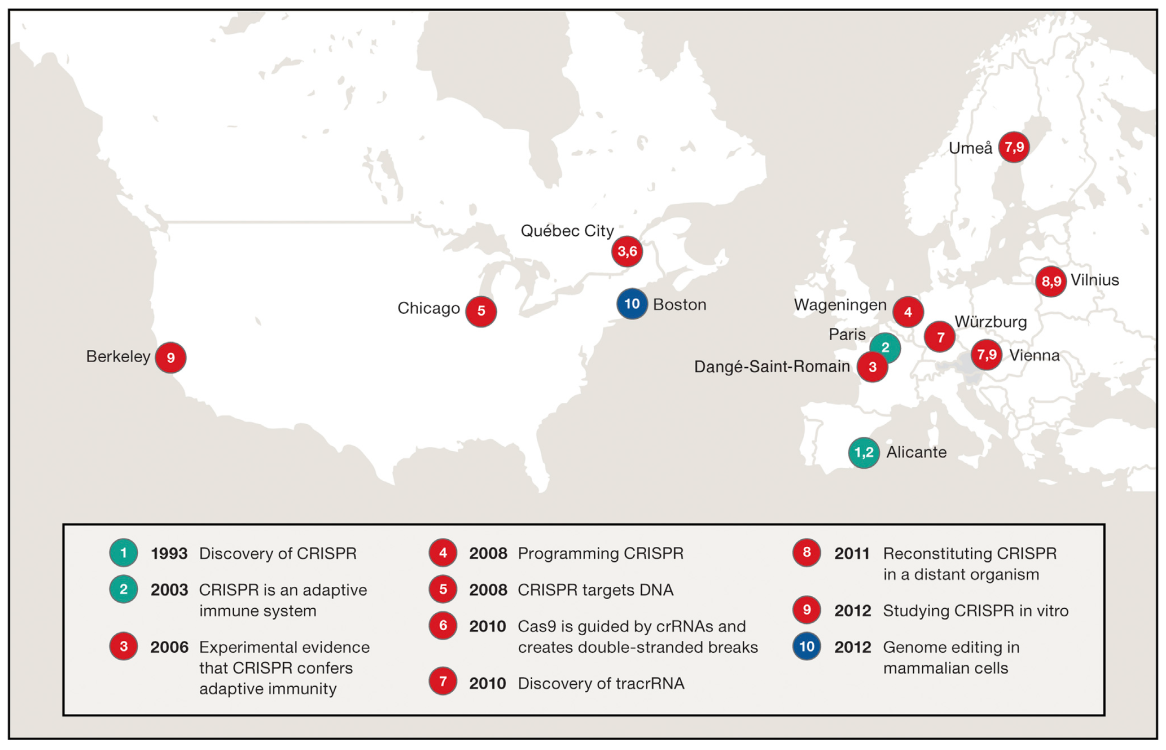
\includegraphics[width=0.8\textwidth]{Map.png}
    \caption{}
    \label{fig:my_label}
\end{figure}


Dans tous les cas, les grandes orientations ou tendances de la recherche sont souvent définis aux niveaux des états, en privilégiant certains secteurs d'activité.









\subsection{Les financements}




Dans de grandes universités américaines comme Princeton, qui est privée, il y a, à l'intérieur des instituts (facultés), des centres dédiés à des thématiques spécifiques financés directement par des donateurs (Effron, Bezos). Il y a aussi des chaires de professeurs "James S. McDonnell Distinguished University Professorship in Physics". Un chercheur peut très bien être financé par des bourses d'organismes publics (NSF, NIH...) ou privés (Mellon, Alfred Sloan, Gates), mais aussi cas un peu plus rare par des entreprises (Merck, Google), pour faire de la recherche conjointe.   

Dans une université comme Paris Saclay, le ratio financements publics privé sera plus important qu'à Princeton, et sera surtout le fait de financements nationaux et européens. Il va sans dire qu'en terme de dotation globale Princeton qui a un budget se chiffrant en milliard de dollards est beaucoup plus riche que Paris Saclay. Avec des fonds pareils, ils disposent de bureaux d'investissements, qui 
investissent dans le capital risque.
Les 5 plus grands fonds d'investissements universitaires sont respectivement Harvard (53 milliards), University of Texas System (45), Yale (40), Stanford (36) et Princeton (33).
A titre de comparaison le PIB de la Belgique en 2022 était de de 583 et celui du Mozambique de 18 milliards de dollars. Harvard compte environ 23000 étudiants, 14000 employés et 2500 professeurs. La Belgique compte  
12 millions de personnes et le Mozambique 34.

https://www.investopedia.com/articles/markets/081616/top-5-largest-university-endowments.asp


\subsection{Les revues de recherche}

Exemple de NEuron, cosyne.

Cout de publier dans une revue de 

\subsection{Les conférences}



\section{Conclusion}
J'ai voulu expliquer ce que faire de la recherche concrètement veut dire, c'est à dire le quotidien des chercheurs, et j'ai aussi voulu expliquer.

see \citep{Snake}).


%\bibliographystyle{unsrtnat}
%\bibliography{references}


\bibliographystyle{plain}
\bibliography{references}



\end{document}


